% Options for packages loaded elsewhere
\PassOptionsToPackage{unicode}{hyperref}
\PassOptionsToPackage{hyphens}{url}
\PassOptionsToPackage{dvipsnames,svgnames,x11names}{xcolor}
%
\documentclass[
]{article}

\usepackage{amsmath,amssymb}
\usepackage{setspace}
\usepackage{iftex}
\ifPDFTeX
  \usepackage[T1]{fontenc}
  \usepackage[utf8]{inputenc}
  \usepackage{textcomp} % provide euro and other symbols
\else % if luatex or xetex
  \usepackage{unicode-math}
  \defaultfontfeatures{Scale=MatchLowercase}
  \defaultfontfeatures[\rmfamily]{Ligatures=TeX,Scale=1}
\fi
\usepackage{lmodern}
\ifPDFTeX\else  
    % xetex/luatex font selection
\fi
% Use upquote if available, for straight quotes in verbatim environments
\IfFileExists{upquote.sty}{\usepackage{upquote}}{}
\IfFileExists{microtype.sty}{% use microtype if available
  \usepackage[]{microtype}
  \UseMicrotypeSet[protrusion]{basicmath} % disable protrusion for tt fonts
}{}
\makeatletter
\@ifundefined{KOMAClassName}{% if non-KOMA class
  \IfFileExists{parskip.sty}{%
    \usepackage{parskip}
  }{% else
    \setlength{\parindent}{0pt}
    \setlength{\parskip}{6pt plus 2pt minus 1pt}}
}{% if KOMA class
  \KOMAoptions{parskip=half}}
\makeatother
\usepackage{xcolor}
\usepackage[top=2cm,bottom=2cm,left = 2.5cm,right = 2.5cm]{geometry}
\setlength{\emergencystretch}{3em} % prevent overfull lines
\setcounter{secnumdepth}{5}
% Make \paragraph and \subparagraph free-standing
\ifx\paragraph\undefined\else
  \let\oldparagraph\paragraph
  \renewcommand{\paragraph}[1]{\oldparagraph{#1}\mbox{}}
\fi
\ifx\subparagraph\undefined\else
  \let\oldsubparagraph\subparagraph
  \renewcommand{\subparagraph}[1]{\oldsubparagraph{#1}\mbox{}}
\fi


\providecommand{\tightlist}{%
  \setlength{\itemsep}{0pt}\setlength{\parskip}{0pt}}\usepackage{longtable,booktabs,array}
\usepackage{calc} % for calculating minipage widths
% Correct order of tables after \paragraph or \subparagraph
\usepackage{etoolbox}
\makeatletter
\patchcmd\longtable{\par}{\if@noskipsec\mbox{}\fi\par}{}{}
\makeatother
% Allow footnotes in longtable head/foot
\IfFileExists{footnotehyper.sty}{\usepackage{footnotehyper}}{\usepackage{footnote}}
\makesavenoteenv{longtable}
\usepackage{graphicx}
\makeatletter
\def\maxwidth{\ifdim\Gin@nat@width>\linewidth\linewidth\else\Gin@nat@width\fi}
\def\maxheight{\ifdim\Gin@nat@height>\textheight\textheight\else\Gin@nat@height\fi}
\makeatother
% Scale images if necessary, so that they will not overflow the page
% margins by default, and it is still possible to overwrite the defaults
% using explicit options in \includegraphics[width, height, ...]{}
\setkeys{Gin}{width=\maxwidth,height=\maxheight,keepaspectratio}
% Set default figure placement to htbp
\makeatletter
\def\fps@figure{htbp}
\makeatother

\usepackage{stmaryrd}
\usepackage{multicol}
\usepackage{graphicx}
\usepackage{ragged2e}
\usepackage{animate, dsfont, here, xspace}
%\usepackage{tikz}
\usepackage{tikz,pgfplots}
 \pgfplotsset{compat=1.17}
%\includepdf[fitpaper=true, pages=-]{img/pdg.pdf}


\DeclareMathOperator{\e}{e}
\DeclareMathOperator{\Determinant}{det}
\renewcommand{\P}{\mathds{P}} %Apparement \P existe déjà ?
\newcommand\N{\mathds{N}}
\newcommand\Norm{\mathcal{N}}
\newcommand\R{\mathds{R}}
\newcommand\Z{\mathds{Z}}
\newcommand\transp[1]{{#1}^T}
%\newcommand\C{\mathds{C}}
%\newcommand\Z{\mathds{Z}}


\newcommand\1{\mathds{1}}
\newcommand{\E}[2][]{{\mathds{E}}_{#1}
  \def\temp{#2}\ifx\temp\empty
  \else
    \left[#2\right]
  \fi
}
\newcommand{\V}[2][]{{\mathds{V}}_{#1}
  \def\temp{#2}\ifx\temp\empty
  \else
    \left[#2\right]
  \fi
}
\newcommand\ud{\,\mathrm{d}}
\newcommand{\ps}[2]{\left\langle #1 \,,\, #2 \right\rangle}

% blocks
\usepackage{environ}
\usepackage[tikz]{bclogo}

\tikzstyle{titlestyle} =[draw=black!80,fill=black!20, text=black,
 right=10pt, rounded corners]
\mdfdefinestyle{symmaryboxstyle}{
	linecolor=black!80, backgroundcolor = black!5,
	skipabove=\baselineskip, innertopmargin=\baselineskip,
	innerbottommargin=\baselineskip,
	userdefinedwidth=\textwidth,
	middlelinewidth=1.2pt, roundcorner=5pt,
	skipabove={\dimexpr0.5\baselineskip+\topskip\relax},
	frametitleaboveskip=\dimexpr-\ht\strutbox\relax,
	innerlinewidth=0pt,
}
\newcounter{summarybox}
\NewEnviron{summary_box}[2][true]{%
\refstepcounter{summarybox} % on incrémente le compteur
\begin{mdframed}[style=symmaryboxstyle,
nobreak=#1,
frametitle={%
      \tikz[baseline=(current bounding box.east),outer sep=0pt]
      \node[titlestyle,anchor=east]
    {Encadré \thesummarybox{} --- #2};}
]
\vspace{-0.5em}
\BODY
\end{mdframed}
}

\usepackage{amsthm}
%\theoremstyle{remark}
\newtheorem*{remarque}{Remarque}

\usepackage{mathrsfs}
\usepackage{fontawesome5}

%\usepackage[style=authoryear,%,uniquename=false, uniquelist=false,
%maxbibnames=2]{biblatex-chicago}
% \usepackage[options]{natbib}
% \bibliographystyle{chicago}

%\DefineBibliographyStrings{english}{andothers={et\addabbrvspace alii}}
\usepackage[authordate16,backend=biber,maxcitenames=2]{biblatex-chicago}
\usepackage{booktabs}
\usepackage{longtable}
\usepackage{array}
\usepackage{multirow}
\usepackage{wrapfig}
\usepackage{float}
\usepackage{colortbl}
\usepackage{pdflscape}
\usepackage{tabu}
\usepackage{threeparttable}
\usepackage{threeparttablex}
\usepackage[normalem]{ulem}
\usepackage{makecell}
\usepackage{xcolor}
\makeatletter
\@ifpackageloaded{caption}{}{\usepackage{caption}}
\AtBeginDocument{%
\ifdefined\contentsname
  \renewcommand*\contentsname{Table of contents}
\else
  \newcommand\contentsname{Table of contents}
\fi
\ifdefined\listfigurename
  \renewcommand*\listfigurename{List of Figures}
\else
  \newcommand\listfigurename{List of Figures}
\fi
\ifdefined\listtablename
  \renewcommand*\listtablename{List of Tables}
\else
  \newcommand\listtablename{List of Tables}
\fi
\ifdefined\figurename
  \renewcommand*\figurename{Figure}
\else
  \newcommand\figurename{Figure}
\fi
\ifdefined\tablename
  \renewcommand*\tablename{Table}
\else
  \newcommand\tablename{Table}
\fi
}
\@ifpackageloaded{float}{}{\usepackage{float}}
\floatstyle{ruled}
\@ifundefined{c@chapter}{\newfloat{codelisting}{h}{lop}}{\newfloat{codelisting}{h}{lop}[chapter]}
\floatname{codelisting}{Listing}
\newcommand*\listoflistings{\listof{codelisting}{List of Listings}}
\makeatother
\makeatletter
\makeatother
\makeatletter
\@ifpackageloaded{caption}{}{\usepackage{caption}}
\@ifpackageloaded{subcaption}{}{\usepackage{subcaption}}
\makeatother
\ifLuaTeX
  \usepackage{selnolig}  % disable illegal ligatures
\fi
\usepackage{bookmark}

\IfFileExists{xurl.sty}{\usepackage{xurl}}{} % add URL line breaks if available
\urlstyle{same} % disable monospaced font for URLs
\hypersetup{
  pdftitle={Supplemental material},
  colorlinks=true,
  linkcolor={blue},
  filecolor={Maroon},
  citecolor={Blue},
  urlcolor={Blue},
  pdfcreator={LaTeX via pandoc}}

\title{Supplemental material}
\author{}
\date{}

\begin{document}
\maketitle

\setstretch{2}
\appendix

\section{Coefficients, gain and phase shift functions}\label{sec-an-cof}

\begin{figure}

\caption{\label{fig-graphs-coef-lc}Coefficients, gain and phase shift
functions for the Linear-Constant (LC) filter with \(I/C=3.5\).}

\centering{

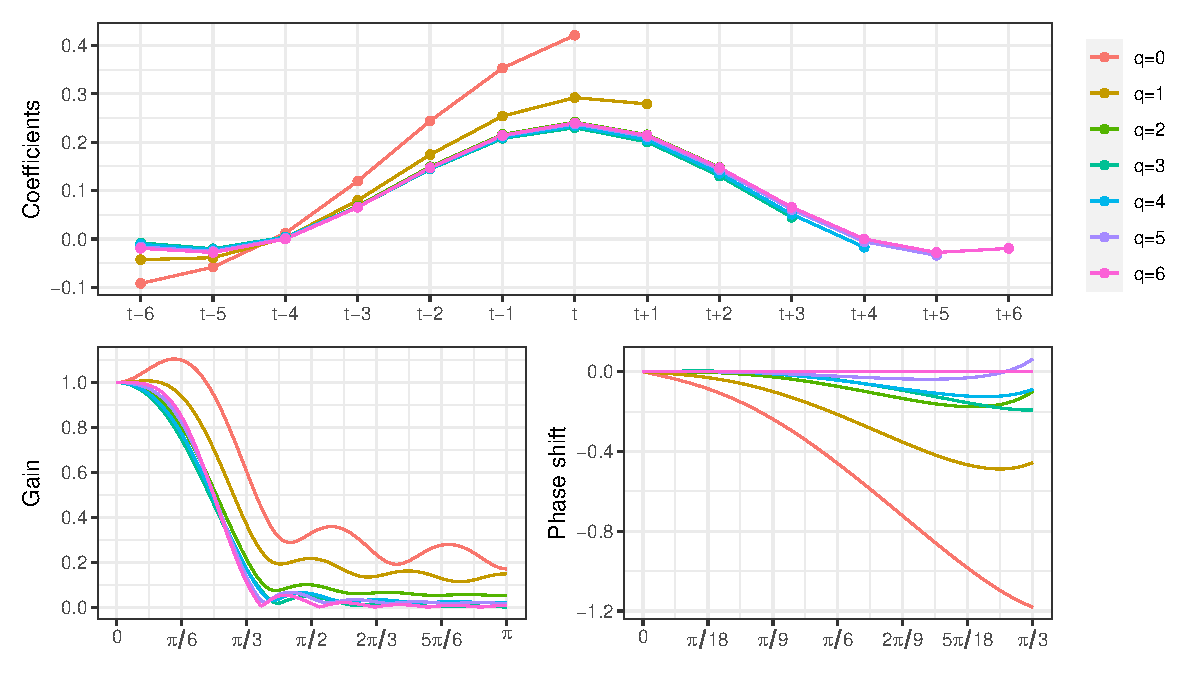
\includegraphics[width=1\textwidth,height=\textheight]{img/filters_used/lc.pdf}

}

\end{figure}%

\begin{figure}

\caption{\label{fig-graphs-coef-ql}Coefficients, gain and phase shift
functions for the Quadratic-Linear (QL) filter with \(I/C=3.5\).}

\centering{

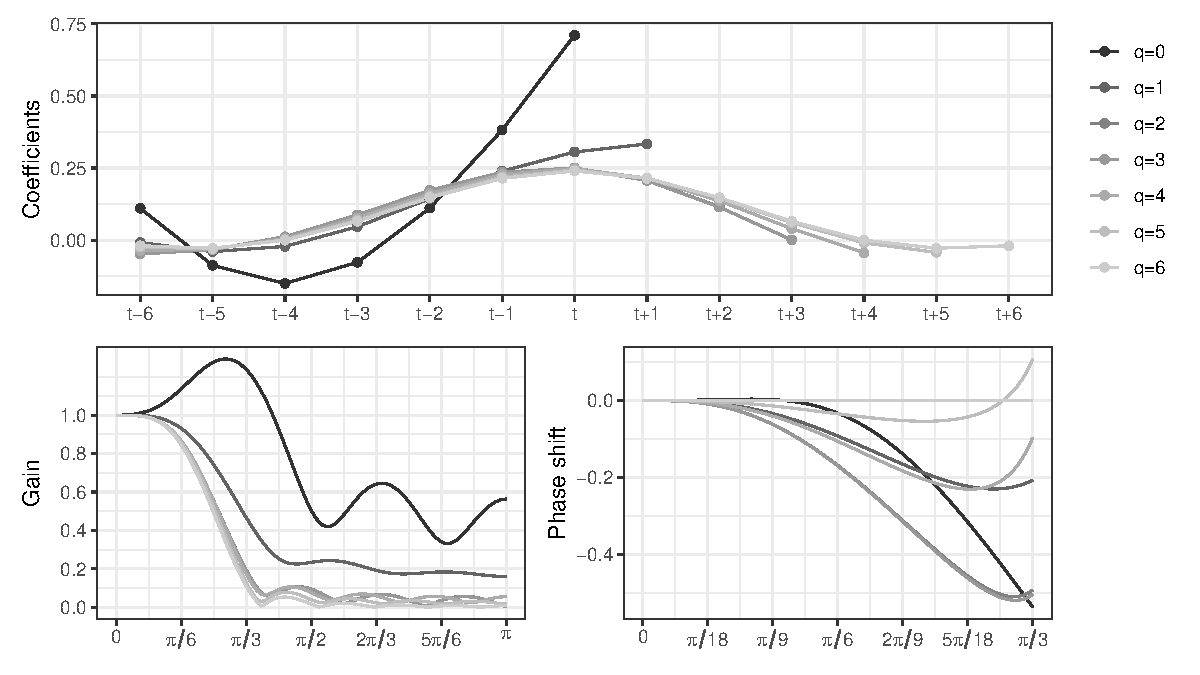
\includegraphics[width=1\textwidth,height=\textheight]{img/filters_used/ql.pdf}

}

\end{figure}%

\begin{figure}

\caption{\label{fig-graphs-coef-cq}Coefficients, gain and phase shift
functions for the Cubic-Quadratic (CQ) filter with \(I/C=3.5\).}

\centering{

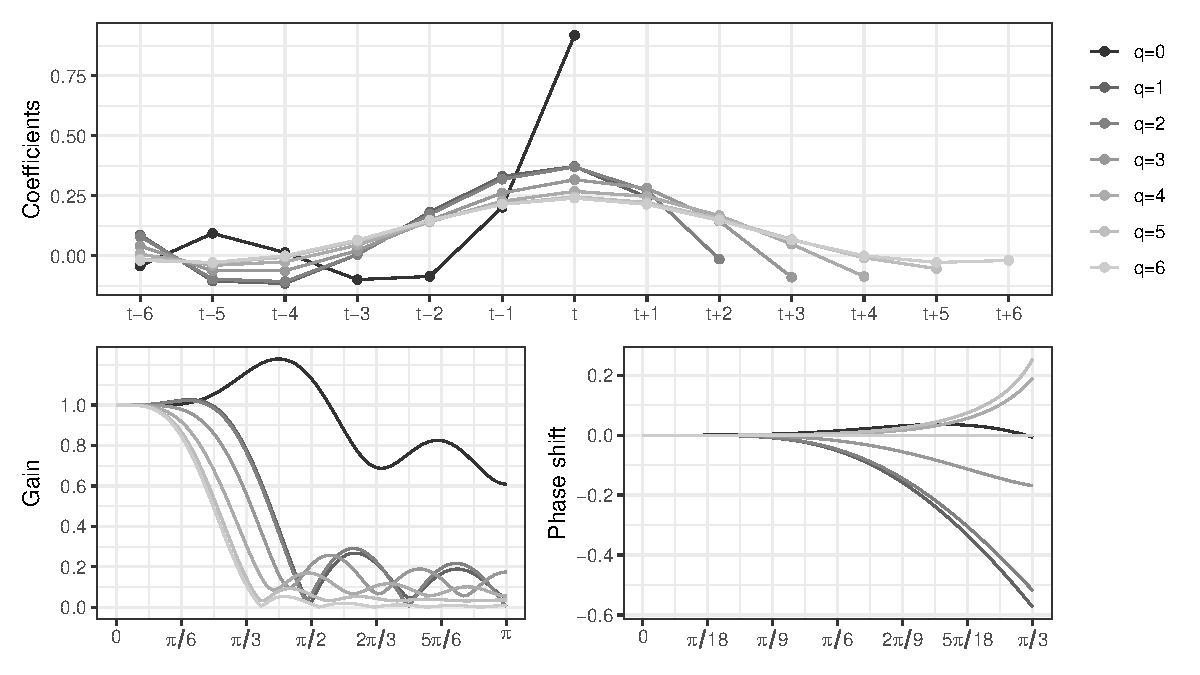
\includegraphics[width=1\textwidth,height=\textheight]{img/filters_used/cq.pdf}

}

\end{figure}%

\begin{figure}

\caption{\label{fig-graphs-coef-daf}Coefficients, gain and phase shift
functions for the direct asymmetric filter (DAF).}

\centering{

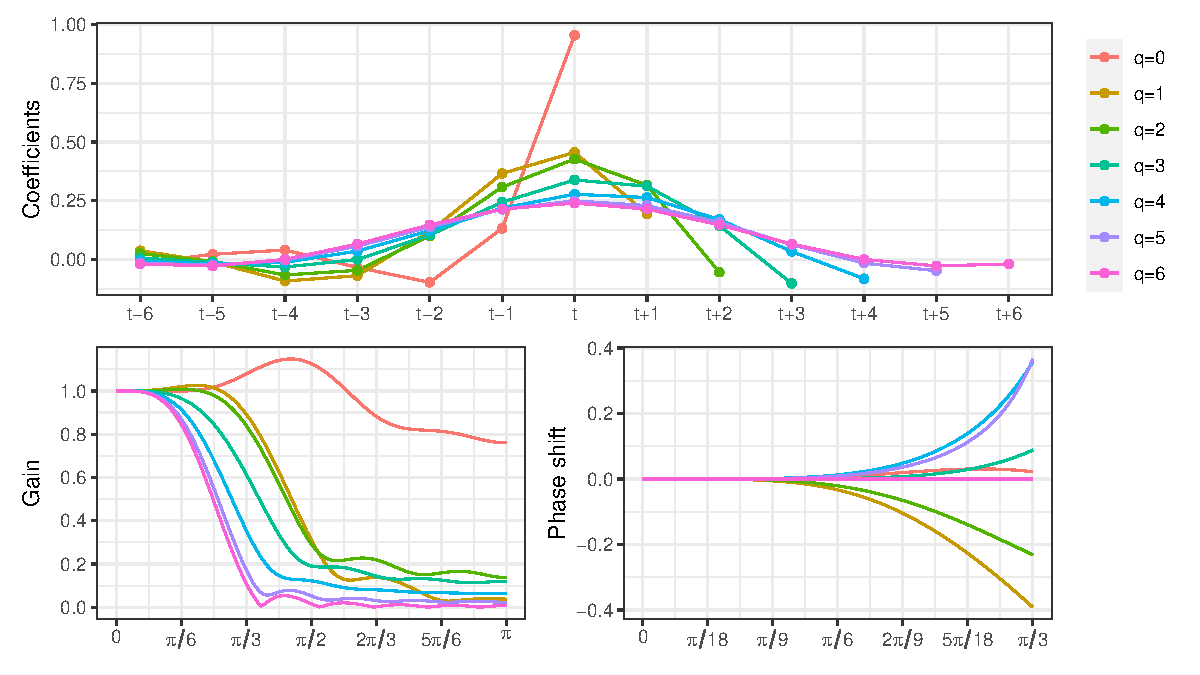
\includegraphics[width=1\textwidth,height=\textheight]{img/filters_used/daf.pdf}

}

\end{figure}%

\newpage

\section{Different specifications for the estimation of the slope and
concavity}\label{different-specifications-for-the-estimation-of-the-slope-and-concavity}

\begin{figure}

\caption{\label{fig-graphs-lc-deg-final}Distribution of phase shift
associated to the local parametrisation of the linear-constant (LC)
filter using the final estimates of \(\delta/\sigma\), by the bandwidth
\(h\) of the henderson filter used to estimate \(\sigma\) and the degree
\(d\) of the trend to estimate \(\delta\).}

\centering{

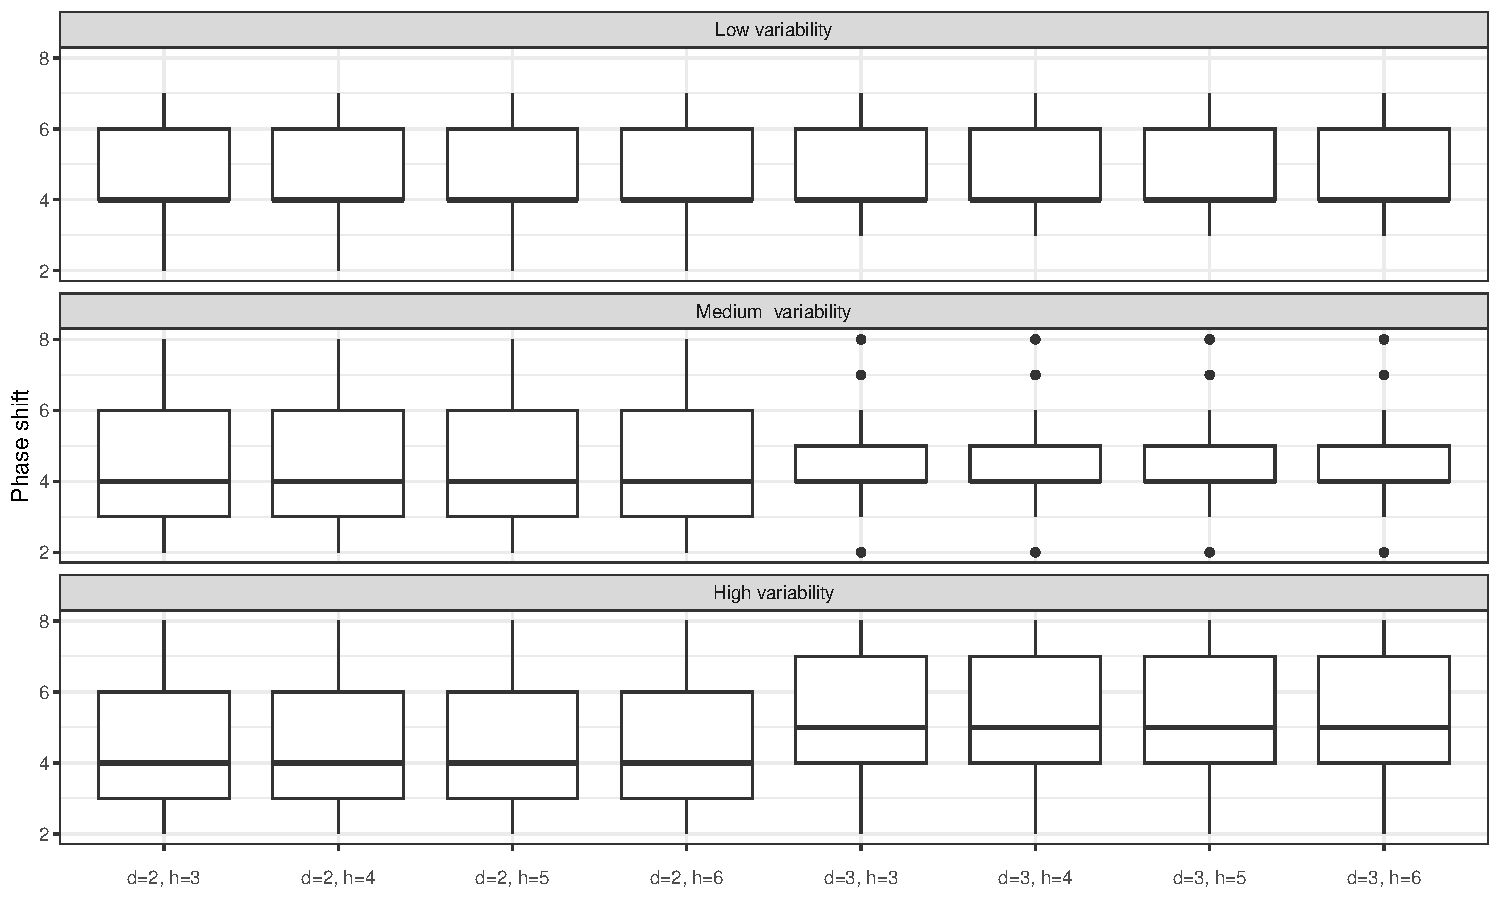
\includegraphics[width=1\textwidth,height=\textheight]{img/simulations/phase_shift_simul_local_final_lc.pdf}

}

\end{figure}%

\begin{figure}

\caption{\label{fig-graphs-lc-deg}Distribution of phase shift associated
to the local parametrisation of the linear-constant (LC) filter using
the final estimates of \(\delta/\sigma\), by the bandwidth \(h\) of the
henderson filter used to estimate \(\sigma\) and the degree \(d\) of the
trend to estimate \(\delta\).}

\centering{

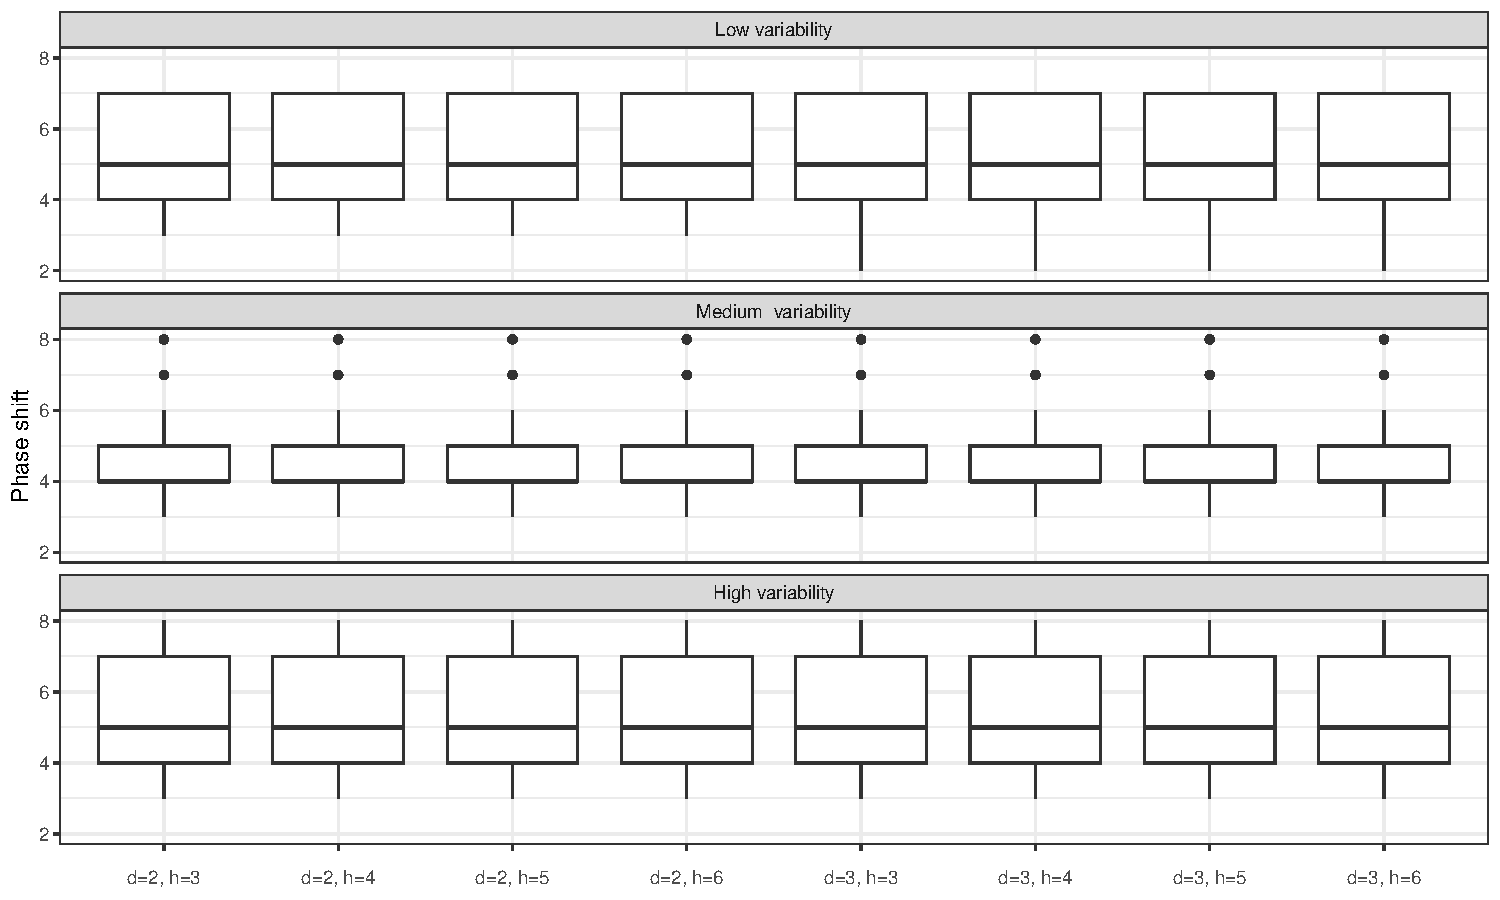
\includegraphics[width=1\textwidth,height=\textheight]{img/simulations/phase_shift_simul_local_lc.pdf}

}

\end{figure}%

\begin{figure}

\caption{\label{fig-graphs-ql-deg-final}Distribution of phase shift
associated to the local parametrisation of the quadratic-linear (QL)
filter using real-time estimates of \(\delta/\sigma\), by the bandwidth
\(h\) of the henderson filter used to estimate \(\sigma\) and the degree
\(d\) of the trend to estimate \(\delta\).}

\centering{

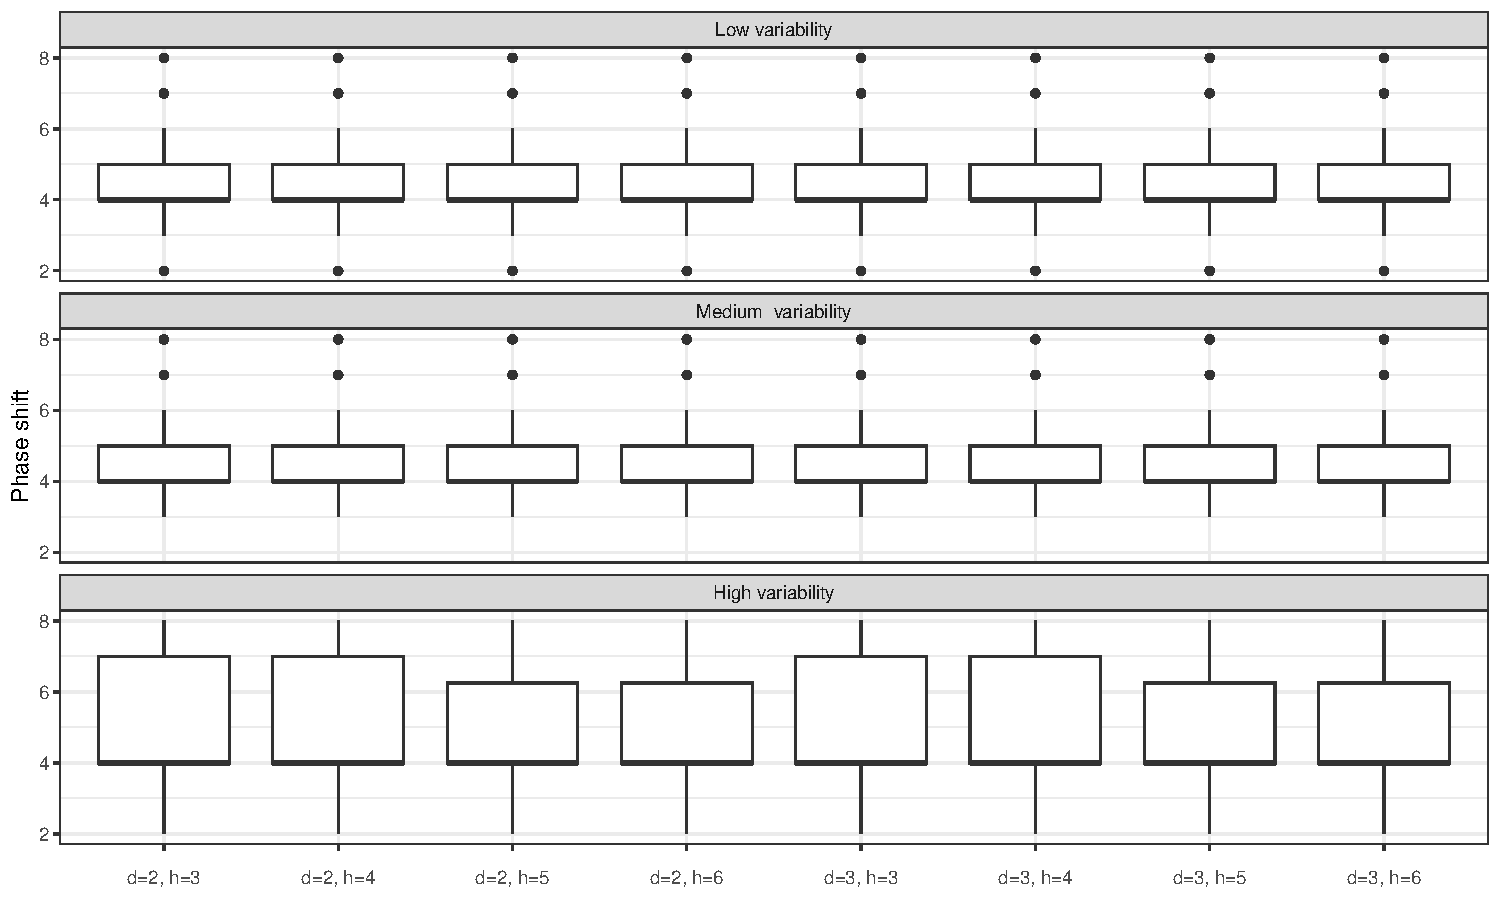
\includegraphics[width=1\textwidth,height=\textheight]{img/simulations/phase_shift_simul_local_final_ql.pdf}

}

\end{figure}%

\begin{figure}

\caption{\label{fig-graphs-ql-deg}Distribution of phase shift associated
to the local parametrisation of the quadratic-linear (QL) filter using
real-time estimates of \(\delta/\sigma\), by the bandwidth \(h\) of the
henderson filter used to estimate \(\sigma\) and the degree \(d\) of the
trend to estimate \(\delta\).}

\centering{

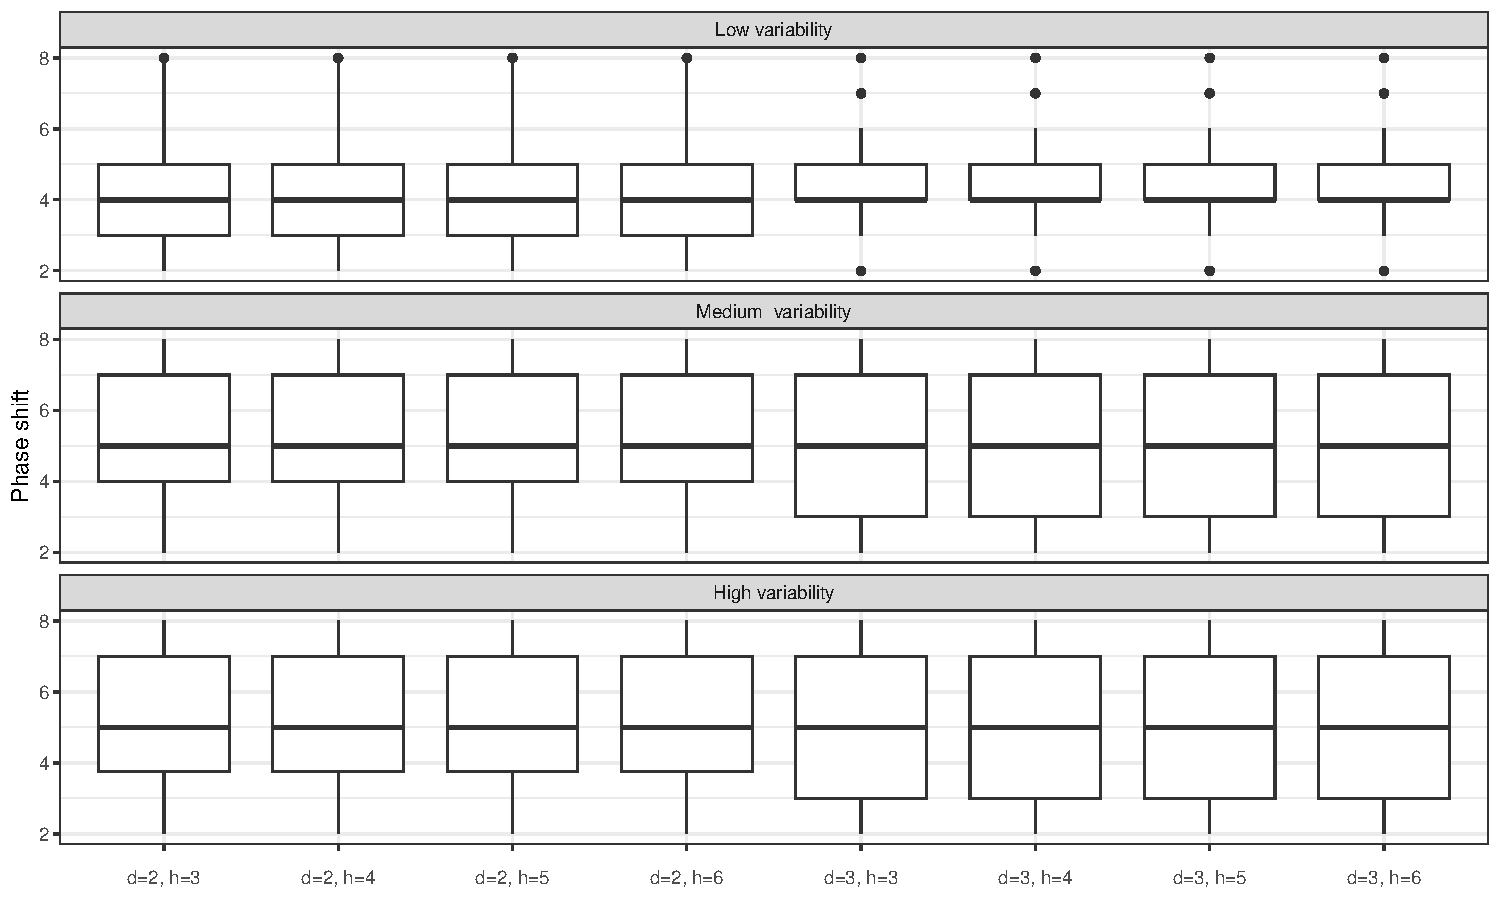
\includegraphics[width=1\textwidth,height=\textheight]{img/simulations/phase_shift_simul_local_ql.pdf}

}

\end{figure}%

\newpage

\section{Impact of the span used to detect the ARIMA
model}\label{impact-of-the-span-used-to-detect-the-arima-model}

\begin{figure}

\caption{\label{fig-graphs-impact-span}Distribution of phase shift on
simulated series by number of years used to identify and estimate the
ARIMA model.}

\centering{

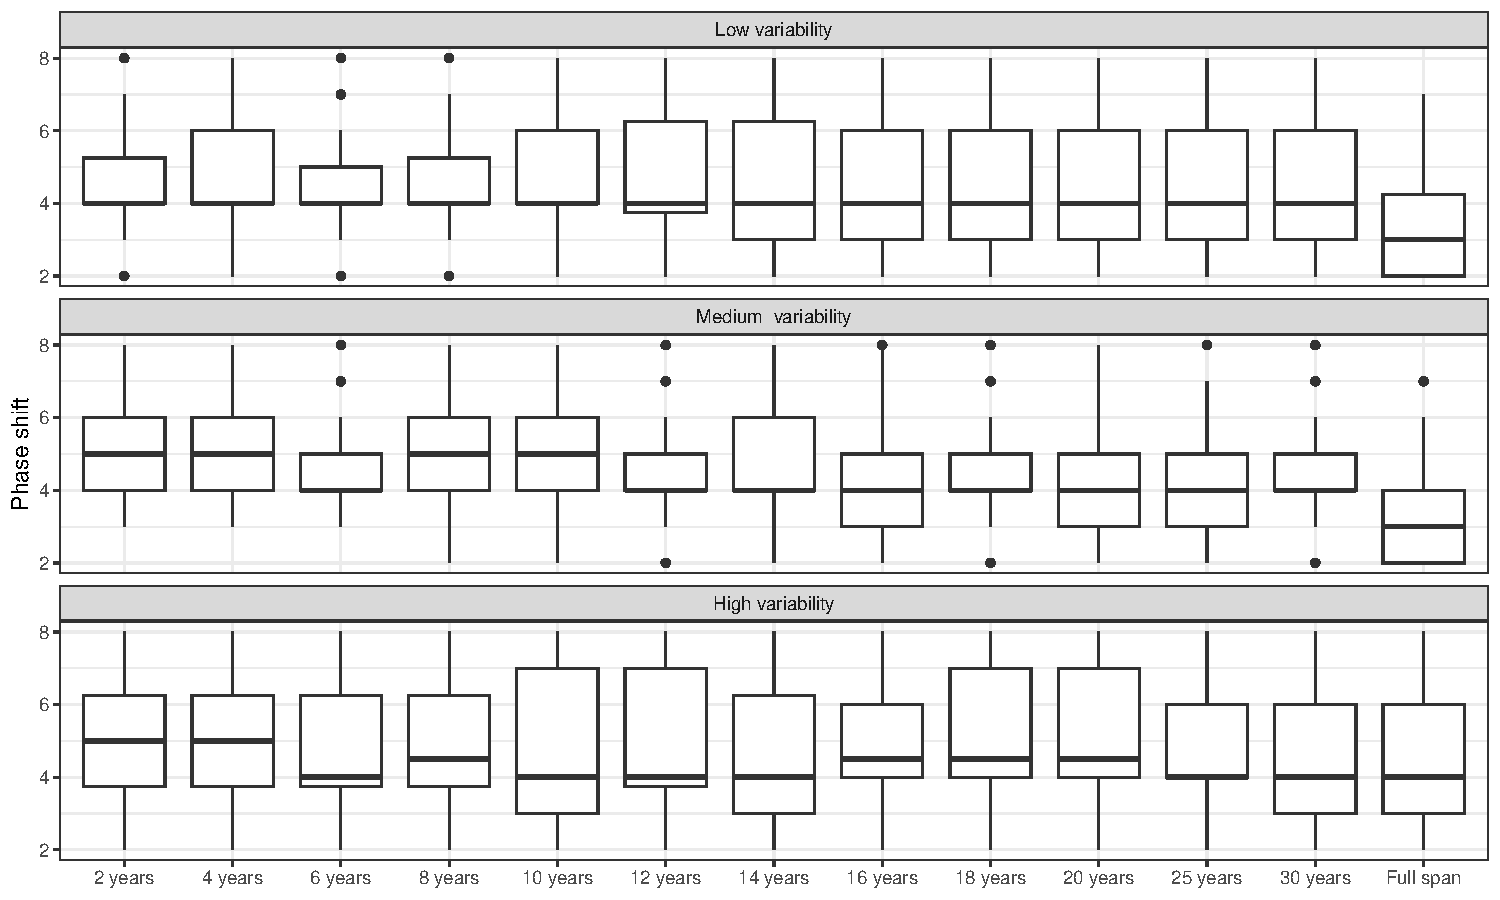
\includegraphics[width=1\textwidth,height=\textheight]{img/simulations/phase_shift_simul_arima_length.pdf}

}

\end{figure}%

\newpage

\section{Nearest neighbour bandwidth}\label{nearest-neighbour-bandwidth}

\begin{figure}

\caption{\label{fig-graphs-coef-lc-nn}Coefficients, gain and phase shift
functions for the Linear-Constant (LC) filter with \(I/C=3.5\) and a
nearest neighbour bandwidth.}

\centering{

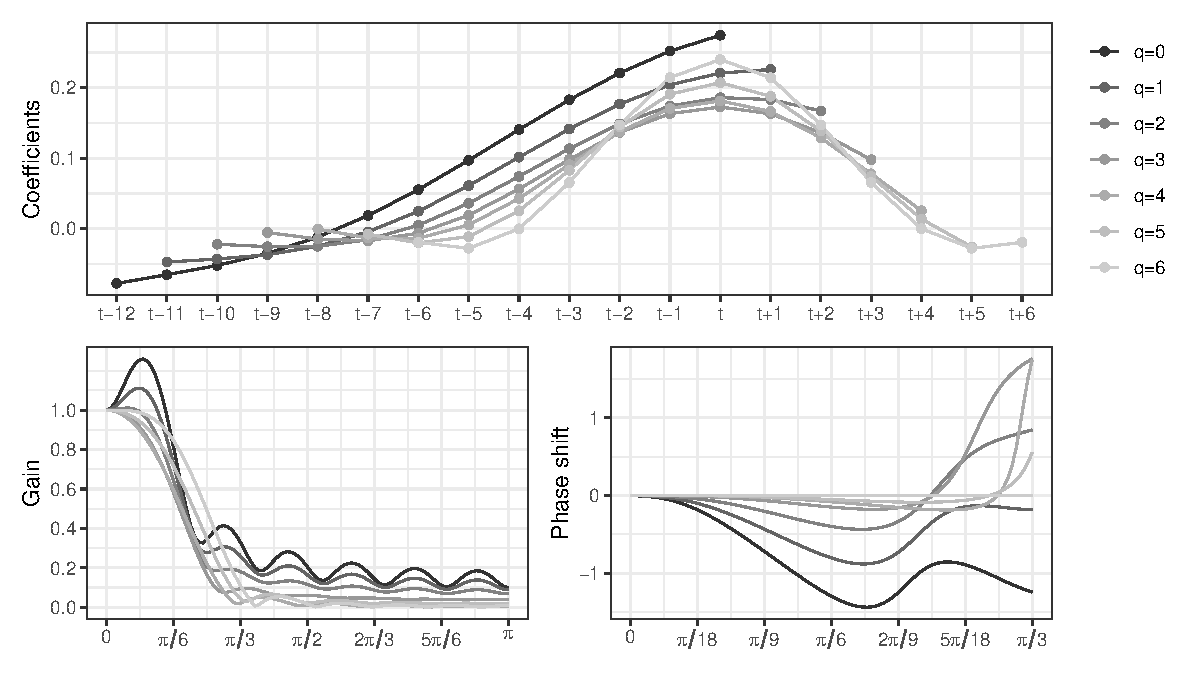
\includegraphics[width=1\textwidth,height=\textheight]{img/filters_used/lc_nn.pdf}

}

\end{figure}%

\begin{figure}

\caption{\label{fig-graphs-coef-ql-nn}Coefficients, gain and phase shift
functions for the Quadratic-Linear (QL) filter with \(I/C=3.5\) and a
nearest neighbour bandwidth.}

\centering{

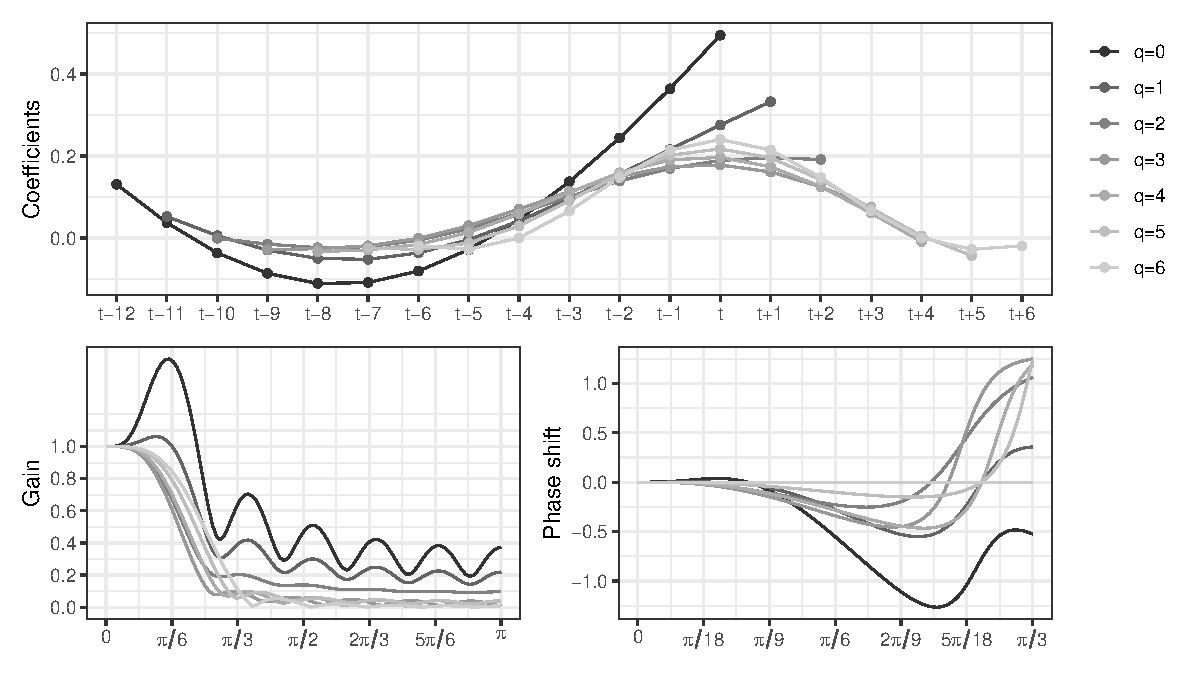
\includegraphics[width=1\textwidth,height=\textheight]{img/filters_used/ql_nn.pdf}

}

\end{figure}%

\begin{figure}

\caption{\label{fig-graphs-coef-cq-nn}Coefficients, gain and phase shift
functions for the Cubic-Quadratic (CQ) filter with \(I/C=3.5\) and a
nearest neighbour bandwidth.}

\centering{

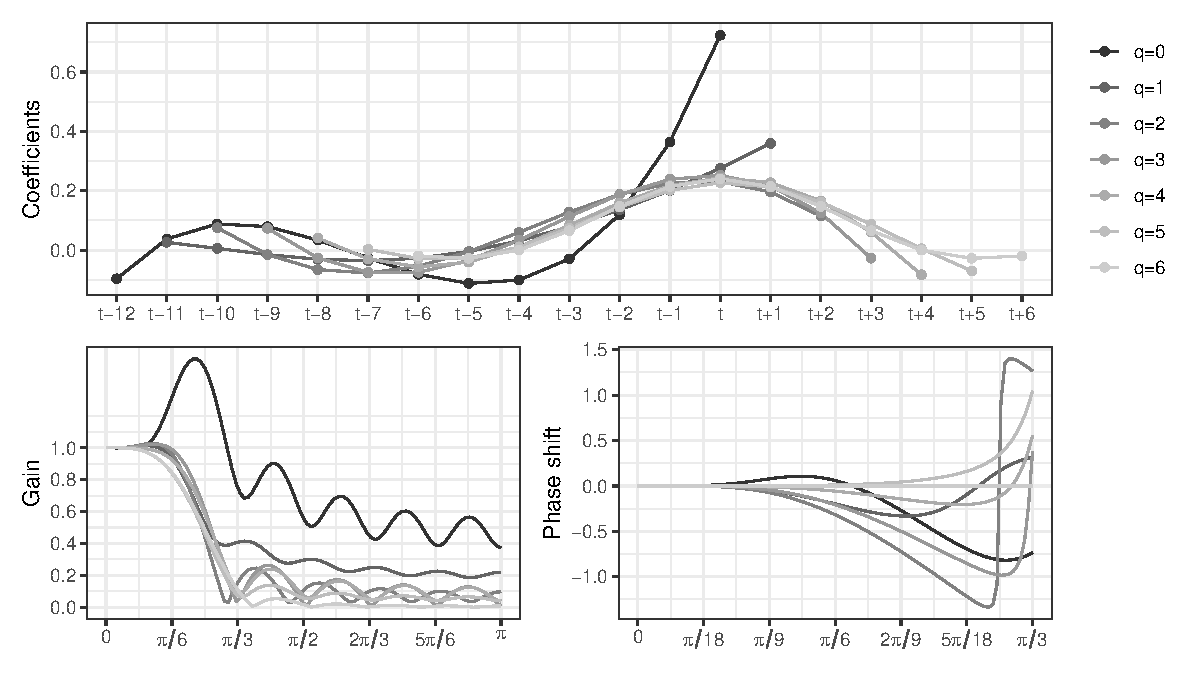
\includegraphics[width=1\textwidth,height=\textheight]{img/filters_used/cq_nn.pdf}

}

\end{figure}%

\begin{figure}

\caption{\label{fig-graphs-coef-daf-nn}Coefficients, gain and phase
shift functions for the direct asymmetric filter (DAF) with a nearest
neighbour bandwidth.}

\centering{

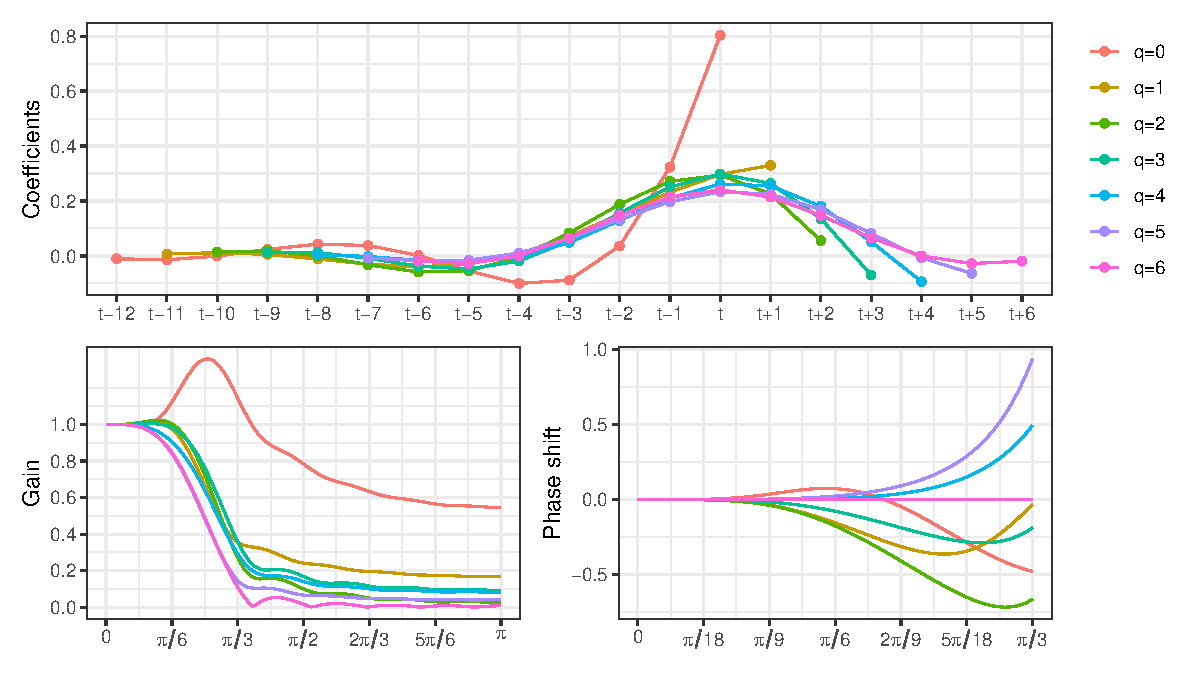
\includegraphics[width=1\textwidth,height=\textheight]{img/filters_used/daf_nn.pdf}

}

\end{figure}%

\begin{figure}

\caption{\label{fig-nn-lp}Distribution of phase shift using nearest
neighbour bandwidth.}

\centering{

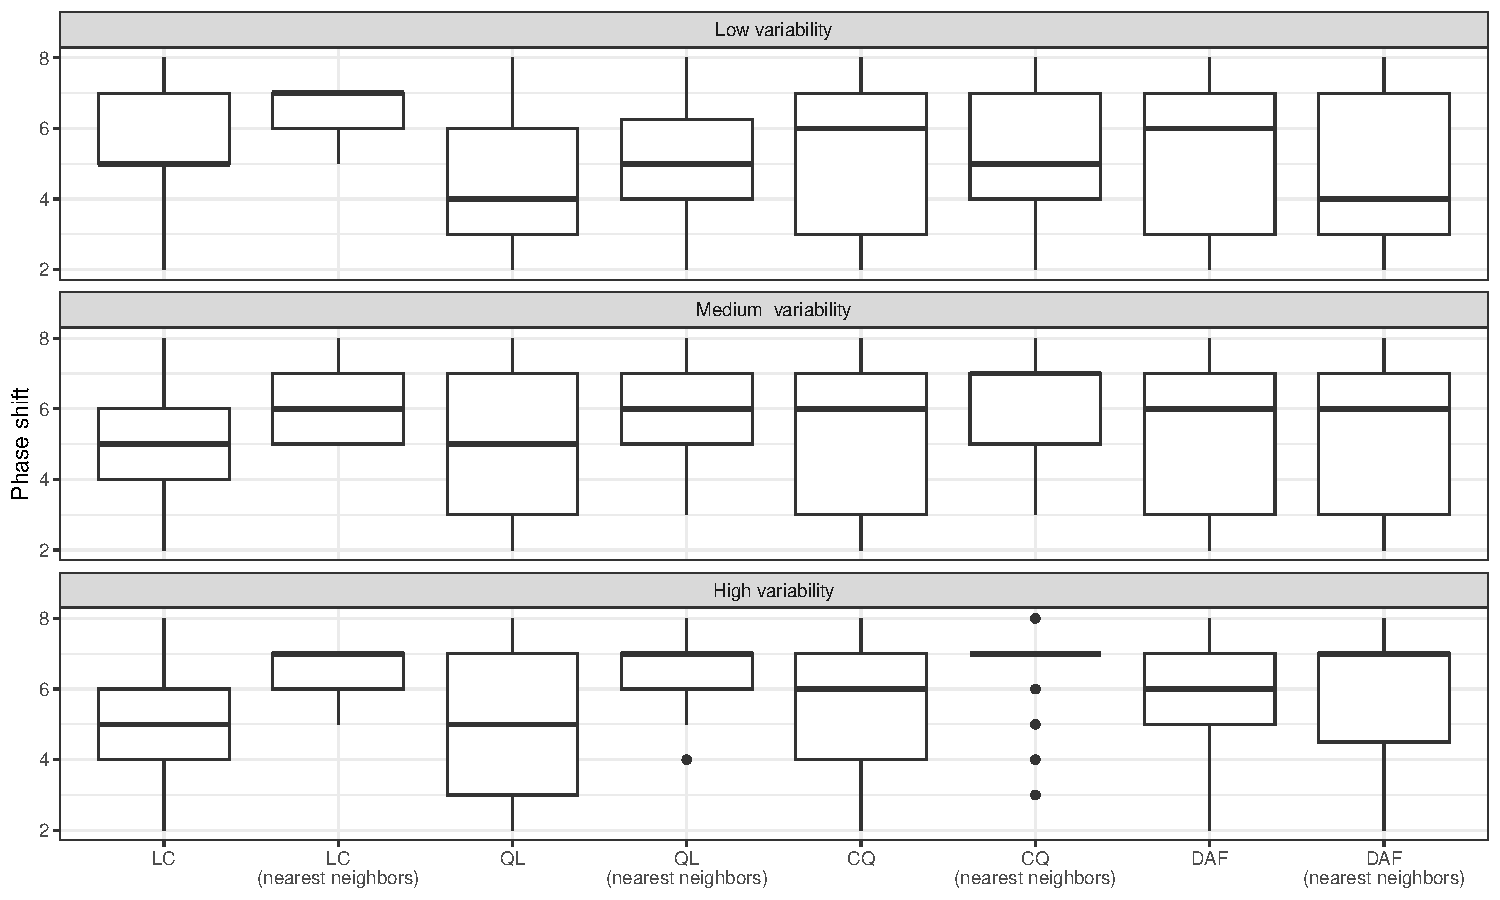
\includegraphics[width=1\textwidth,height=\textheight]{img/simulations/phase_shift_simul_nn_lp.pdf}

}

\end{figure}%

\begin{figure}

\caption{\label{fig-nn-localparam}Distribution of phase shift using
nearest neighbour bandwidth for polynomial filters with local
parametrisation.}

\centering{

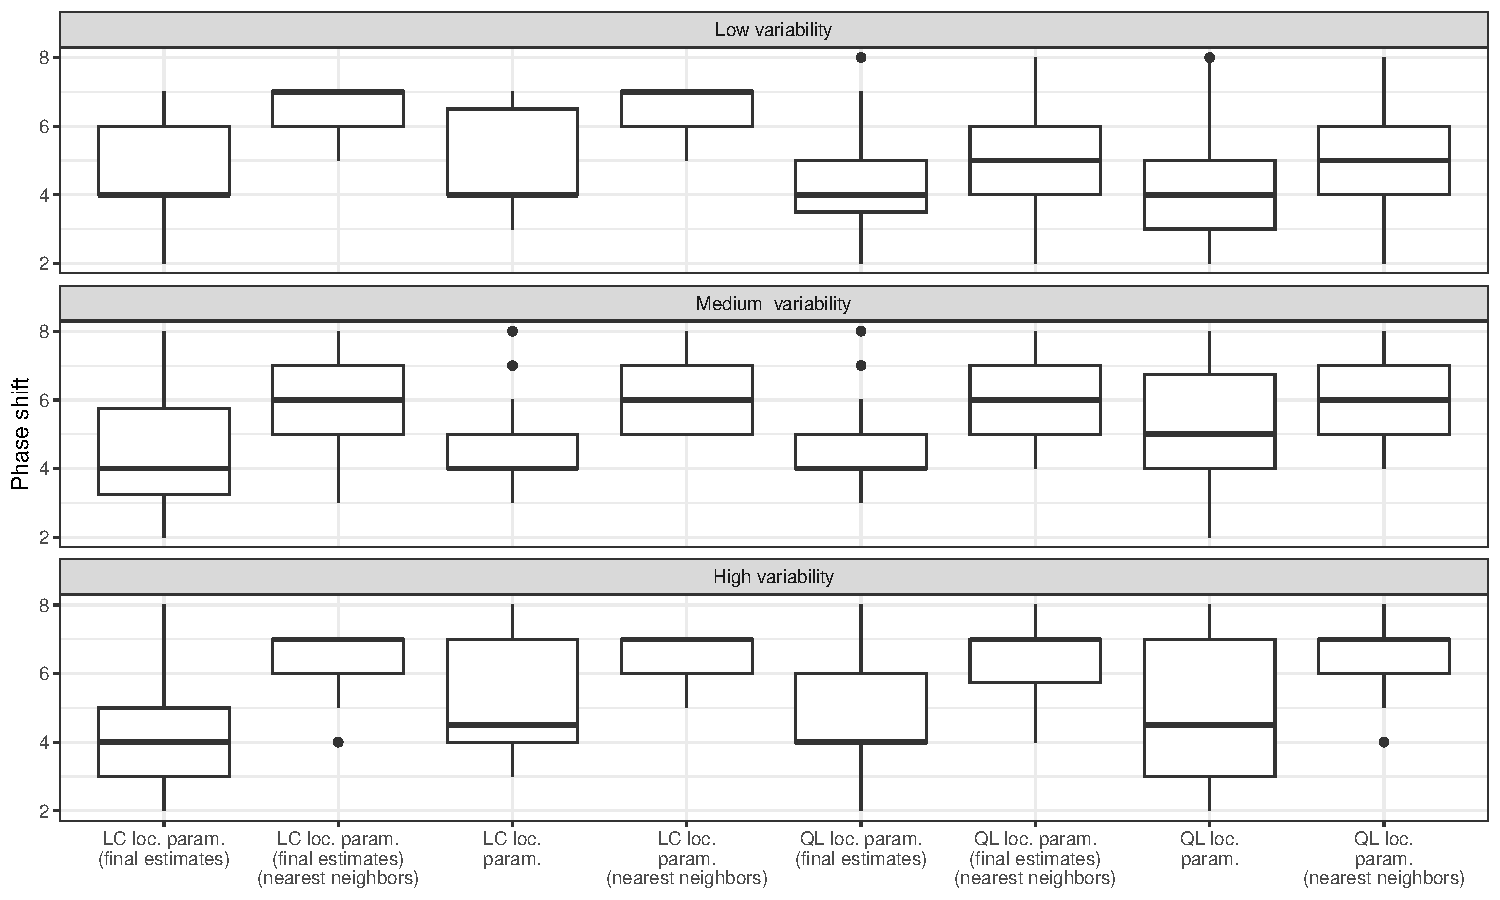
\includegraphics[width=1\textwidth,height=\textheight]{img/simulations/phase_shift_simul_nn_lp_localparam.pdf}

\justifying

\emph{Note: nearest bandwidth moving average are used to estimate slope
and concavity.} \emph{We thus do not distinguish local parametrisation
and final local parametrisation which asumptions might not be
plausible.} \emph{Indeed, using the same framework as for fixed
bandwidth, the final local parametrisation for real-time estimates would
implie modelling a polynomial of degree 2 or 3 other 25 months (which
doesn't seem plausible).}

}

\end{figure}%

\newpage

\section{Quarterly data}\label{quarterly-data}

\begin{figure}

\caption{\label{fig-graphs-quarterly}Distribution of phase shift on
quarterly data.}

\centering{

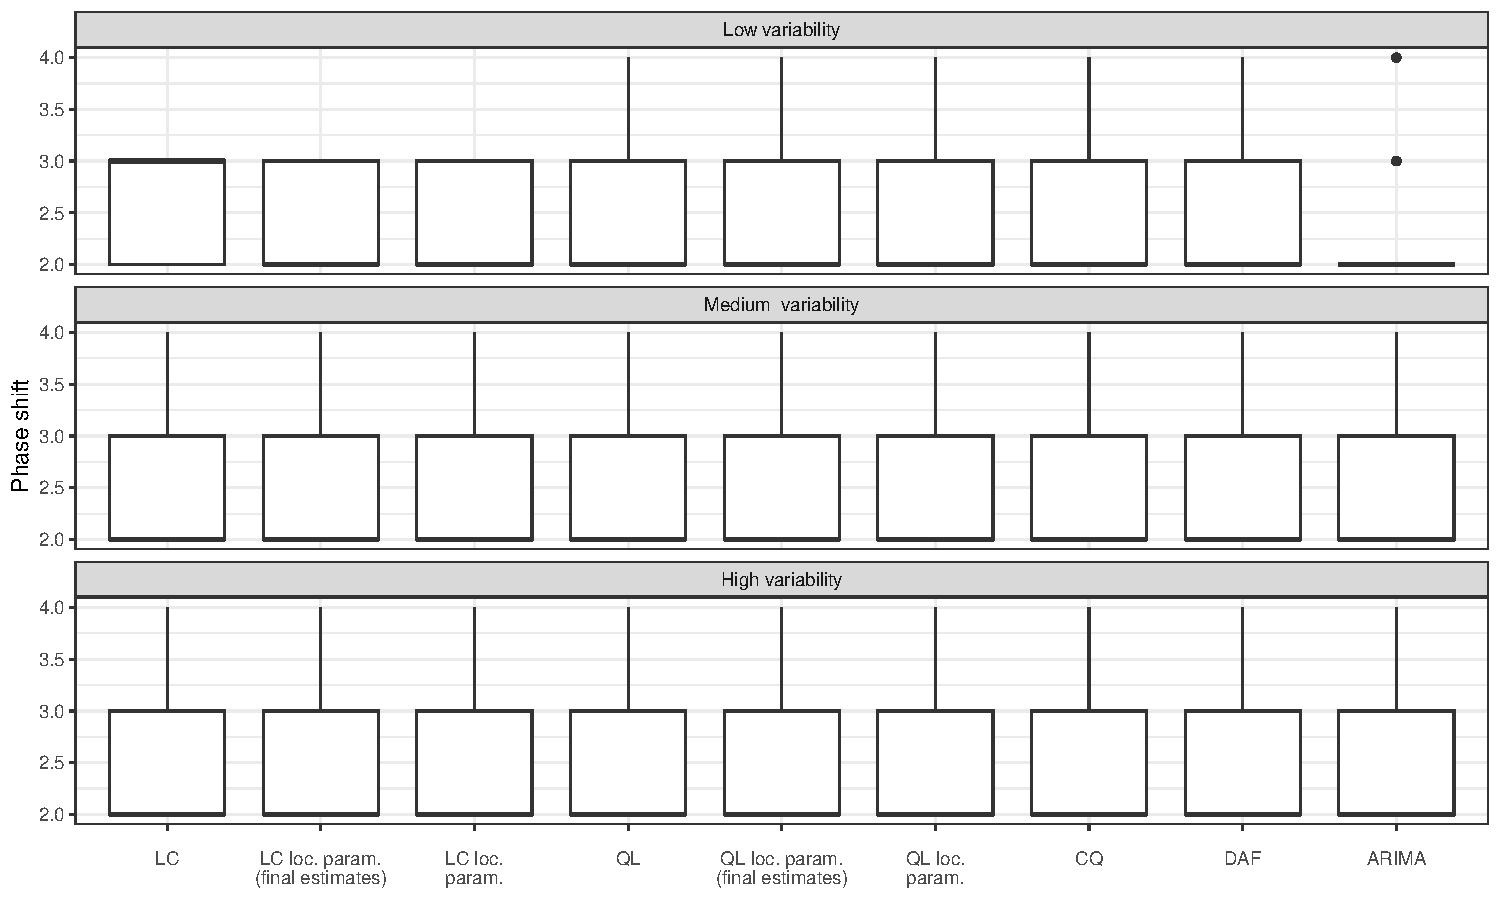
\includegraphics[width=1\textwidth,height=\textheight]{img/simulations/phase_shift_simul_q.pdf}

}

\end{figure}%

\begin{table}

\caption{\label{tbl-simulrev-q}Average of the relative deviations of the
revisions for the different filters on simulated quarterly series with
medium variability.}

\centering{

\begin{tabular}{ccc}
\toprule
Method & $q=0$ & $q=1$\\
\midrule
\addlinespace[0.3em]
\multicolumn{3}{l}{\textbf{$MAE_{fe}(q) = \mathbb E\left[\left|(TC_{t|t+q} -  TC_{t|last})/TC_{t|last}\right|\right]$}}\\
\hspace{1em}LC & 0.76 & 0.11\\
\hspace{1em}LC local param. (final estimates) & 0.73 & 0.11\\
\hspace{1em}LC local param. & 0.71 & 0.12\\
\hspace{1em}QL & 0.93 & 0.46\\
\hspace{1em}QL local param. (final estimates) & 0.58 & 0.12\\
\hspace{1em}QL local param. & 0.97 & 0.33\\
\hspace{1em}CQ & 1.15 & 1.02\\
\hspace{1em}DAF & 1.15 & 0.43\\
\hspace{1em}ARIMA & 0.49 & 0.26\\
\addlinespace[0.3em]
\multicolumn{3}{l}{\textbf{$MAE_{ce}(q)=\mathbb E\left[
\left|(TC_{t|t+q} - TC_{t|t+q+1})/TC_{t|t+q+1}\right|
\right]$}}\\
\hspace{1em}LC & 0.36 & 0.11\\
\hspace{1em}LC local param. (final estimates) & 0.32 & 0.11\\
\hspace{1em}LC local param. & 0.34 & 0.12\\
\hspace{1em}QL & 1.75 & 0.46\\
\hspace{1em}QL local param. (final estimates) & 0.23 & 0.12\\
\hspace{1em}QL local param. & 0.40 & 0.33\\
\hspace{1em}CQ & 0.07 & 1.02\\
\hspace{1em}DAF & 0.75 & 0.43\\
\hspace{1em}ARIMA & 0.27 & 0.26\\
\bottomrule
\end{tabular}

}

\end{table}%



\end{document}
